\documentclass[xcolor=dvipsnames,aspectratio=169]{beamer}

% INCLUSIÓN DOS PAQUETES IMPRESCINDIBLES DE IDIOMA E CODIFICACIÓN DE CARACTERE.
\usepackage[T1]{fontenc}
\usepackage[english]{babel}
\usepackage[utf8]{inputenc}
\usepackage{csquotes}

%ACRONYMS para engadir un glosario de acronimos automatizado
% \usepackage[acronyms,nonumberlist,nopostdot,nomain,nogroupskip]{glossaries}
% \input{./acronyms.tex}

% PAQUETES PARA FIGURAS E GRAFICOS
\usepackage{graphicx}
%   \usepackage[pdftex]{graphicx}
  \usepackage{epstopdf}
   \graphicspath{{./img/}}
  % and their extensions so you won't have to specify these with
  % every instance of \includegraphics
   \DeclareGraphicsExtensions{.eps,.pdf,.png,.jpg}   
\usepackage{subfigure}
\usepackage{caption}
\usepackage[inkscapelatex=false]{svg}


%Tikz plots
\usepackage{tikz}
\usepackage{tikzscale}
\usetikzlibrary{plotmarks,patterns,decorations.pathreplacing,backgrounds,calc,arrows,arrows.meta,spy,matrix,backgrounds,shapes,math}

\usepackage{pgfplots}
\pgfplotsset{compat=newest}
\pgfplotsset{plot coordinates/math parser=false}
\usepgfplotslibrary{patchplots,groupplots,fillbetween}

% OUTROS PAQUETES DE USO COMUN. HOXE EN DIA OS COMPILADORES SON TAN RAPIDOS QUE EU METO TODOS SEMPRE
% \usepackage{float}
% \usepackage{ucs} 
% \usepackage{subcaption}
\usepackage{psfrag}
\usepackage{verbatim}
\usepackage{amsmath}
\usepackage{amsfonts}
\usepackage{amssymb}
\usepackage{amsthm}
\usepackage{pifont}
\usepackage{array}
\usepackage{listings}
\usepackage{stfloats}
\usepackage{algorithm} 
\usepackage{algorithmic} 
\usepackage{url} 
\usepackage{enumerate}
\usepackage{multirow}
\usepackage{wasysym}
\usepackage{cancel}
\usepackage{lmodern}

\usepackage{mathrsfs}  

% DECLARACION DAS FONTES DA UVIGO
\usepackage[sfdefault]{roboto}
\usepackage{librebaskerville}
\setbeamerfont{title}{family=\librebaskerville,size=\Huge}
\setbeamerfont{subtitle}{family=\librebaskerville,size=\large}
% IMPORTANTE: a fonte 'campus' non queda ben para títulos de papers academicos,ç
% pero se de verdade se desexa empregar, seguir os seguintes pasos
% 1) Instalar o comando otftotfm en linux
% 2) sudo otftotfm -a -e texnansx campus_bold.otf CampusBold
% 3) asegurarse que o ficheiro auxiliar ./EETtemplateFiles/fonts/T1CampusBold.df está no directorio de traballo
% 4) descomentar a liña abaixo e comentar a liña que lle asigna librebaskerville arriba
\input{EETtemplateFiles/fonts/T1CampusBold.df}
\setbeamerfont{title}{family=\fontfamily{CampusBold},size=\Huge}

% DETLARACIÓN DO TEMA A USAR
% 
% ESTES TEMAS TEÑEN CABECEIRAS MOI GRANDES
% \usetheme{Berkeley} %large titlebar w/side dossier
% \usetheme{PaloAlto} 
% \usetheme{Copenhagen} %large titlebar w/2 side index
% \usetheme{Antibes} %large titlebar w/tree
% \usetheme{Singapore} %large titlebar w/balls evanescent
% \usetheme{Berlin} %large titlebar w/balls solid
% \usetheme{Dresden} %same as above with different color boxing
% \usetheme{Rochester} %large tittle-only titlebar
% ESTES TEMAS TEÑEN CABECEIRAS MEDIANAS
% \usetheme{CambridgeUS} %title titlebar w/current section
% \usetheme{Malmoe} %title titlebar w/current section Copenhagen style
% \usetheme{Madrid} %title titlebar w/page counter footer
% ESTES TEMAS TEÑEN CABECEIRAS DELGADAS
% \usetheme{Frankfurt} %small titlebar w/ progress balls
% \usetheme{metropolis} %metal
% ESTES TEMAS NON TEÑEN CABECEIRA DE COR, PERO SI TITULO SOBRE BRANCO
% \usetheme{Boadilla} %sombras e decoracion
\usetheme{Pittsburgh} %rectangulos planos
% ESTES TEMAS TEÑEN INDICES OU INFO NUNHA BARRA LATERAL GRANDE
% \usetheme{Goettingen} %right dossier evanescent
% \usetheme{Marburg} %right dossier fading to black
% \usetheme{Bergen} %notebook

%aspect modifiers
\useinnertheme{circles} %this makes item lists nicer
% \useoutertheme{infolines} %toggle thin info borders


% DECLARACIÓN DA COMBINACIÓN DE CORES A USAR. SE NON SE ESPECIFICA NADA TOMA A DEFINIDA POR DEFECTO
\definecolor{EETblue}{HTML}{0094e0} % a mate dark blue
\usecolortheme[named=EETblue]{structure} % EET UVigo blue
% outros temas de cores de beamer
% \usecolortheme{seagull} %makes title boxes gray color with blackr
% \usecolortheme{spruce} %makes title boxes pastel blue - gray color
% cores internos (items)
% \usecolortheme[named=Red]{structure} 
% \usecolortheme[named=Green]{structure} 
% \usecolortheme[named=OliveGreen]{structure} 
% \usecolortheme[named=PineGreen]{structure} 
% \usecolortheme[named=TealBlue]{structure} 
% \usecolortheme[named=SeaGreen]{structure}
% \usecolortheme[RGB={00,78,135}]{structure} % a dark cobalt blue 
% \usecolortheme[RGB={155,0,20}]{structure} % a slighlty darkened mate red

% MODIFICACIONS DAS CORES PARA A PAXINA DE TITULO SIMILAR Á OFICIAL
\setbeamercolor*{title}{use=structure,fg=structure.bg, bg=structure.fg}  
\setbeamercolor*{subtitle}{use=structure,fg=white}  
\setbeamercolor*{author}{use=structure,fg=structure.fg}
% \setbeamercolor*{institute}{use=structure,fg=structure.fg}
\setbeamercolor*{date}{use=structure,fg=structure.fg}
\setbeamertemplate{frametitle}[default][left]

% MODIFICACIONS DA SIDEBAR E FOOTLINE PARA INCLUIR AS IMAXES CORPORATIVAS.
\setbeamertemplate{footline}[text line]{%
  \parbox{\linewidth}{
    %ESTE TEXTO DA FOOTLINE PODESE MODIFICAR A GUSTO -----------------------------------------
    \insertshorttitle\hfill\insertshortauthor\hfill\insertpagenumber / \inserttotalframenumber
    %----------------------------------------------------------------------------------------
    \hfill
  
\includegraphics[width=.15\paperwidth,trim={0 2.5cm 3.5cm .75cm},clip]{EETtemplateFiles/img/Logotipo_ESCOLA.pdf}\vspace*{2pt}}}
\setbeamersize{sidebar width left = .10\paperwidth}
\setbeamertemplate{sidebar canvas left}{}
\setbeamertemplate{sidebar left}{%
  \vspace*{\fill}
  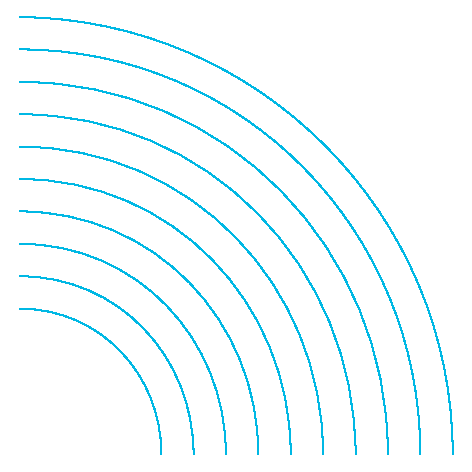
\includegraphics[width=.15\paperwidth,height=.15\paperwidth]{EETtemplateFiles/img/Simbolo_ESCOLA.pdf}\\
  
\includegraphics[width=.15\paperwidth,trim={.4cm .5cm .4cm 2.25cm},clip]{EETtemplateFiles/img/Logotipo_ESCOLA.pdf}
  \vspace*{-11pt}%
}

% MATH SYMBOLS

\newcommand{\field}[1]{\mathbb{#1}}

\DeclareMathOperator{\atan}{atan}
\DeclareMathOperator{\acos}{acos}
\DeclareMathOperator{\asin}{asin}

% \newcommand{\mb}[1]{\mathbf{#1}}


\newcommand{\A}{\mathbf{A}}
\newcommand{\B}{\mathbf{B}}
\newcommand{\Cb}{\mathbf{C}}
\newcommand{\D}{\mathbf{D}}
\newcommand{\Eb}{\mathbf{E}}
\newcommand{\F}{\mathbf{F}}
\newcommand{\Gb}{\mathbf{G}}
\newcommand{\Hb}{\mathbf{H}}
\newcommand{\I}{\mathbf{I}}
\newcommand{\J}{\mathbf{J}}
\newcommand{\Kb}{\mathbf{K}}
\newcommand{\Lb}{\mathbf{L}}
\newcommand{\M}{\mathbf{M}}
\newcommand{\N}{\mathbf{N}}
\newcommand{\Ob}{\mathbf{O}}
\newcommand{\Pb}{\mathbf{P}}
\newcommand{\Q}{\mathbf{Q}}
\newcommand{\R}{\mathbf{R}}
\newcommand{\Sb}{\mathbf{S}}
\newcommand{\T}{\mathbf{T}}
\newcommand{\U}{\mathbf{U}}
\newcommand{\V}{\mathbf{V}}
\newcommand{\W}{\mathbf{W}}
\newcommand{\X}{\mathbf{X}}
\newcommand{\Y}{\mathbf{Y}}
\newcommand{\Z}{\mathbf{Z}}
\newcommand{\Dl}{\mathbf{\boldsymbol{\Delta}}}
\newcommand{\Sg}{\mathbf{\boldsymbol{\Sigma}}}
\newcommand{\Ld}{\mathbf{\boldsymbol{\Lambda}}}
\newcommand{\Ph}{\mathbf{\boldsymbol{\Phi}}}
\newcommand{\Ps}{\mathbf{\boldsymbol{\Psi}}}
\newcommand{\Up}{\mathbf{\boldsymbol{\Upsilon}}}
\newcommand{\Xib}{\mathbf{\boldsymbol{\Xi}}}
% \newcommand{\D}{\mathbf{D}}
\newcommand{\one}{\mathbf{1}}
\newcommand{\zero}{\mathbf{0}}

\newcommand{\ab}{\mathbf{a}}
\newcommand{\bb}{\mathbf{b}}
\newcommand{\cc}{\mathbf{c}}
\newcommand{\dd}{\mathbf{d}}
\newcommand{\e}{\mathbf{e}}
\newcommand{\f}{\mathbf{f}}
\newcommand{\g}{\mathbf{g}}
\newcommand{\h}{\mathbf{h}}
\newcommand{\ib}{\mathbf{i}}
\newcommand{\jb}{\mathbf{j}}
\newcommand{\kb}{\mathbf{k}}
\newcommand{\lb}{\mathbf{\ell}}
\newcommand{\m}{\mathbf{m}}
\newcommand{\n}{\mathbf{n}}
\newcommand{\ob}{\mathbf{o}}
\newcommand{\pp}{\mathbf{p}}
\newcommand{\q}{\mathbf{q}}
\newcommand{\rr}{\mathbf{r}}
\newcommand{\s}{\mathbf{s}}
\newcommand{\uu}{\mathbf{u}}
\newcommand{\vv}{\mathbf{v}}
\newcommand{\w}{\mathbf{w}}
\newcommand{\x}{\mathbf{x}}
\newcommand{\y}{\mathbf{y}}
\newcommand{\z}{\mathbf{z}}
\newcommand{\al}{\mathbf{\boldsymbol{\alpha}}}
\newcommand{\vmu}{\mathbf{\boldsymbol{\mu}}}
\newcommand{\vlambda}{\mathbf{\boldsymbol{\lambda}}}
\newcommand{\vphi}{\mathbf{\boldsymbol{\phi}}}
\newcommand{\vpsi}{\mathbf{\boldsymbol{\psi}}}
\newcommand{\vrho}{\mathbf{\boldsymbol{\rho}}}
\newcommand{\vups}{\mathbf{\boldsymbol{\upsilon}}}
\newcommand{\vxi}{\mathbf{\boldsymbol{\xi}}}

\newcommand{\rank}{\textnormal{rank}}
% \newcommand{\trace}{\textnormal{trace}}
\newcommand{\exptr}{\textnormal{exptr}}
\newcommand{\tr}{\textnormal{tr}}
% \newcommand{\vstack}{\textnormal{vec}}
% \newcommand{\diag}{\textnormal{diag}}
\newcommand{\vstack}[1]{\Xib_{#1}}
\newcommand{\diag}[1]{\Ld_{#1}}
\newcommand{\tnsr}[2]{\underline{\mathsf{#1}}_{#2}}
\newcommand{\tmult}[1]{\underset{#1}{\times}}

\DeclareMathOperator{\Prob}{Prob}
%  |x>
\newcommand{\ket}[1]{\left\vert#1\right\rangle}
%  <x|
\newcommand{\bra}[1]{\left\langle#1\right\vert}
%  <x|y>
\newcommand{\braket}[2]{\left< #1 \vphantom{#2}\,
                        \right\vert\left.\!\vphantom{#1} #2 \right>}
%  <x|a|y>
\newcommand{\sandwich}[3]{\left< #1 \vphantom{#2 #3} \right|
                          #2 \min\left(\vphantom{#1 #2} #3 \right>}

\newcommand{\pd}[2]{\frac{\partial #1}{\partial #2}}
%  d/dt
\newcommand{\ddt}{\frac{d}{dt}}
%  D/Dx
\newcommand{\pdd}[1]{\frac{\partial}{\partial#1}}
%  |x|
\newcommand{\abs}[1]{\left\vert#1\right\vert}
%  k_{x}
\newcommand{\kv}[1]{\mathbf{k}_{#1}}
%  \textnormal{E}_{domain of integration}{variable}
\newcommand{\Ex}[2]{{\mathbb{E}_{#1}\left[#2\right]}}
\newcommand{\CEx}[3]{{\mathbb{E}_{#1}\left[#2|#3\right]}}
\newcommand{\CInf}[3]{{\textnormal{I}\left(#1;#2|#3\right)}}
\newcommand{\Inf}[2]{{\textnormal{I}\left(#1;#2\right)}}
\newcommand{\CEnt}[2]{{\textnormal{H}\left(#1|#2\right)}}
\newcommand{\Ent}[1]{{\textnormal{H}\left(#1\right)}}
\newcommand{\dCEnt}[2]{{\textnormal{h}\left(#1|#2\right)}}
\newcommand{\dEnt}[1]{{\textnormal{h}\left(#1\right)}}

\newcommand{\cmark}{\ding{51}}%
\newcommand{\xmark}{\ding{55}}%
\newcommand{\itempro}{\item[\textcolor{KYJade}{\Large \cmark}]}
\newcommand{\itemcontra}{\item[\textcolor{ARust}{\Large \xmark}]}
\newcommand\Tau{\mathcal{T}}
%Figure and format fixes


\renewcommand{\figurename}{Fig.}
\newcommand{\PESrule}{\noindent\rule{.57\columnwidth}{0.1mm}}

%theroem environments
% If using amsthm package, we need to delete these theorems before giving them our own definition. does not work for theorem
% \let\theorem\relax
\let\definition\relax
\let\lemma\relax
\let\corollary\relax
\let\example\relax
%
% \newtheorem{theorem}{Theorem}
\newtheorem{definition}{Definition}
\newtheorem{lemma}{Lemma}
\newtheorem{corollary}{Corollary}
\newtheorem{conjecture}{Conjecture}
\theoremstyle{plain}
\newtheorem{remark}{Remark}
\newtheorem{proposition}{Proposition}
\newtheorem{example}{Example}
\newtheorem{homework}{Homework}

%Colors
   \definecolor{blueH3}{rgb}{0,.5,1}
   \definecolor{blueH2}{rgb}{0,0.25,0.75}
   \definecolor{blueH1}{rgb}{0,0,0.5}   
   \definecolor{grayOldText}{rgb}{.5,.5,.5}
   \definecolor{VCobalt}{HTML}{005682}
   \definecolor{TZTeal}{HTML}{008080}
   \definecolor{TZTealfaded}{HTML}{F0FFFF}
   \definecolor{KYJade}{HTML}{008151}
   \definecolor{ARust}{HTML}{a10000}
   \definecolor{FFucsia}{HTML}{7000c3}   
   \definecolor{TAMustard}{HTML}{a1a100}
   \definecolor{Tangerine}{HTML}{d45500}
   
   
% Tikz 
% signal block diagram components
\tikzset{
    block/.style = {draw, rectangle, 
        minimum height=1cm, 
        minimum width=1.2cm, align=center},
    input/.style = {coordinate,node distance=1cm},
    output/.style = {coordinate,node distance=2cm},
    arrow/.style={draw, -latex,node distance=1.5cm},
    pinstyle/.style = {pin edge={latex-, black,node distance=1.5cm}},
    sum/.style = {draw, circle, node distance=1cm}
}
\tikzstyle{pinstyle} = [pin edge={to-,thin,black}]
\def\antenna{%
    -- +(0mm,4.0mm) -- +(2.625mm,7.5mm) -- +(-2.625mm,7.5mm) -- +(0mm,4.0mm) -- +(0mm,0mm)
}
% Overlay highlights on top of the page
\newcommand{\markOverlay}[1]{\tikz[overlay,remember picture] \node (#1) {};}
\newcommand{\drawOverlayBox}[4][]{%
    \tikz[overlay,remember picture]{%
        \coordinate (TopLeft)     at ($(#2)+(-0.4em,1.6em)$);
        \coordinate (BottomRight) at ($(#3)+(0.4em,-1.0em)$);
        %
        \path (TopLeft); \pgfgetlastxy{\XCoord}{\IgnoreCoord};
        \path (BottomRight); \pgfgetlastxy{\IgnoreCoord}{\YCoord};
        \coordinate (LabelPoint) at ($(\XCoord,\YCoord)!0.5!(BottomRight)$);
        %
        \draw [red,#1] (TopLeft) rectangle (BottomRight);
        \node [below, #1, fill=none, fill opacity=1] at (LabelPoint) {#4};
    }
}
\newcommand{\drawOverlayLine}[4][]{%
    \tikz[overlay,remember picture]{%
        \draw [red,#1] ($(#2)$) -- node{#4} ($(#3)$);
    }
}
\newcommand{\drawOverlayCircle}[4][]{%
    \tikz[overlay,remember picture]{%
        \draw [red,#1] ($(#2)$) circle (#3) node{#4};
    }
}
   
   %%%%%%%%%%%%%%%%%%%%%%%%%%%%%%%%%%%%%%%%%%%%%%%%%%%%%%%%%%%%%%%%%
%% The following definitions are to extend the LaTeX algorithmic 
%% package with SWITCH statements and one-line structures.
%% The extension is by 
%%   Prof. Farn Wang 
%%   Dept. of Electrical Engineering, 
%%   National Taiwan University. 
%% 
\newcommand{\SWITCH}[1]{\STATE \textbf{switch} (#1)}
\newcommand{\ENDSWITCH}{\STATE \textbf{end switch}}
\newcommand{\CASE}[1]{\STATE \textbf{case} #1\textbf{:} \begin{ALC@g}}
\newcommand{\ENDCASE}{\end{ALC@g}}
\newcommand{\CASELINE}[1]{\STATE \textbf{case} #1\textbf{:} }
\newcommand{\DEFAULT}{\STATE \textbf{default:} \begin{ALC@g}}
\newcommand{\ENDDEFAULT}{\end{ALC@g}}
\newcommand{\DEFAULTLINE}[1]{\STATE \textbf{default:} }
%% 
%% End of the LaTeX algorithmic package extension.

\newcounter{MYtempeqncnt}


%%%%%%%%%%%%%%%%%%%%%%%%%%%%%%%%%%%%%%%
% Commands to recall text later
%%%%%%%%%%%%%%%%%%%%%%%%%%%%%%%%%%%%%%%
\makeatletter
\newcommand\remembertext[2]{% #1 is a key, #2 is the text
  \immediate\write\@auxout{\unexpanded{\global\long\@namedef{mytext@#1}{#2}}}%
  #2%
}
%
\newcommand\recalltext[1]{%
  \ifcsname mytext@#1\endcsname
    \@nameuse{mytext@#1}%
  \else
    ``??''
  \fi
}

%%%%%%%%%%%%%%%%%%%%%%%%%%%%%%%%%%%%%%%%%%%%%%%%%%%%%%%%%%%%%%%%%%%%%%%%%%%%%%%%%%
%%% Paolo Casari: macros for automating section titling and comment formatting %%%
%%%%%%%%%%%%%%%%%%%%%%%%%%%%%%%%%%%%%%%%%%%%%%%%%%%%%%%%%%%%%%%%%%%%%%%%%%%%%%%%%%
\newcounter{myequationcnt}

\newcounter{rcnt}
\newcounter{ccnt}

\newcommand{\newreviewernopagebreak}[1]{\vspace{5em} \setcounter{ccnt}{0}\section*{\normalsize Comments of #1}\vspace{4mm}}

\newcommand{\ThisIsTheEditorNoPageBreak}{\setcounter{ccnt}{0}\section*{\Large Comments of the Editor}\vspace{3mm}}
\newcommand{\ThisIsTheEditor}{\clearpage \ThisIsTheEditorNoPageBreak}
\newcommand{\ThisIsANewReviewerNoPageBreak}[1]{\vspace{5em} \refstepcounter{rcnt}\label{r#1}\setcounter{ccnt}{0}\section*{\Large Comments of Reviewer \arabic{rcnt}}\vspace{3mm}}
\newcommand{\ThisIsANewReviewer}[1]{\clearpage\vspace{-5em} \ThisIsANewReviewerNoPageBreak{#1}}

\newcommand{\edcomment}[1]{
\begin{tcbremark}
\color{VCobalt}
    \refstepcounter{ccnt}\label{e\arabic{ccnt}}\noindent\textbf{\boldmath\emph{Comment E.\arabic{ccnt}:}} #1\vspace{0.2cm}
\end{tcbremark}
}
\newcommand{\refedcomment}[1]{E.\ref{e#1}}

\newcommand{\revcomment}[1]{
\begin{tcbremark}
\color{VCobalt}
\refstepcounter{ccnt}\label{r\arabic{rcnt}c\arabic{ccnt}}\noindent\textbf{\boldmath\emph{Comment \arabic{rcnt}.\arabic{ccnt}:}} #1\vspace{0.2cm}
\end{tcbremark}
}
\newcommand{\refrevcomment}[2]{\ref{r#1}.\ref{r#1c#2}}

% \newcommand{\ouranswer}[1]{\noindent\emph{Answer:} #1\vspace{0.6cm}}
% \newcommand{\citepap}[1]{\vspace{0.33cm}\begin{minipage}{0.05\textwidth} $\phantom{A}$  \end{minipage}\begin{minipage}{0.85\textwidth}\renewcommand{\baselinestretch}{1.15}\small \emph{#1} \end{minipage}\vspace{0.3cm}}

\newlength{\ansspace}
\addtolength{\ansspace}{0.6cm}
\newcommand{\ansbreak}{\vspace{\ansspace}}

\newlength{\stdleftskip}
\addtolength{\stdleftskip}{\leftskip}
\newlength{\stdrightskip}
\addtolength{\stdrightskip}{\rightskip}
\newlength{\citeskip}
\addtolength{\citeskip}{2em}
\newcommand{\oldbaselinestretch}{1.5}

\newcommand{\setcitepapskip}{%
    \leftskip\citeskip %
    \rightskip\citeskip %
    \renewcommand{\baselinestretch}{1.15}\small%
    \vspace{0.6em}%
    \noindent%
}

\newcommand{\resetLRmargins}{%
    \leftskip\stdleftskip %
    \rightskip\stdrightskip %
    \renewcommand{\baselinestretch}{\oldbaselinestretch}\normalsize %
    \vspace{0.6em}
}

\newcommand{\emans}{\emph{Answer:\ }}


%---------------
% LIMIAR
%---------------
%configuracion de opcions de beamer persoais, pero alleas ao estilo

% COMANDO QUE INTRODUCE UNHA DIAPOSITIVA CUN ÍNDICE NO QUE APARECEN VELADAS TÓDALAS SECCIÓNS MENOS A ACTUAL. ÚTIL PARA INTRODUCIR OS TÍPICOS ÍNDICES INTERMEDIOS.
\newcommand{\Inter}{\frame{\tableofcontents[currentsection]}}
\newcommand{\inter}{\frame{\tableofcontents[currentsection,currentsubsection]}}

% Pes de imaxe
\renewcommand{\figurename}{Fig.}
\addto\captionsenglish{\renewcommand{\figurename}{Fig.}}
\setbeamertemplate{caption}[numbered]

%ESTE PAQUETE PERMITE POÑER A BIBLIOGRAFIA AO PE DE PAXINA CON CONFIGURACIONS ESTETICAS PERSOAIS
% \usepackage[style=ieee,doi=false,isbn=false,url=true,backend=bibtex]{biblatex}
% \bibliography{./bibliografia.bib}
% \newrobustcmd*{\footfullcitenomark}{%
%   \AtNextCite{%
%     \let\thefootnote\relax 
%     \let\mkbibfootnote\mkbibfootnotetext
%     }%
%   \footfullcite}

%paquete para engadir notas de guion ao pdf
\usepackage{pgfpages}
% \setbeameroption{show only notes} 
% \setbeameroption{show notes}
% \setbeameroption{show notes on second screen=right}
% DATOS DO DOCUMENTO
\title[CDA]{Advanced Digital Communications}
\subtitle{Session 4: Time-Varying Channels}
\author[FGC]{\underline{Felipe G\'omez-Cuba}}
\institute[GPSC]{
\begin{columns}[T]
\begin{column}{5cm}\centering
Office A-204\\
Wednesday \& Thursday 15:00-18:00\\
\texttt{gomezcuba@gts.uvigo.es}\\
\end{column}
\end{columns}
}

\date{2025}

\begin{document}

% Diapositiva co título
\frame[plain]{\titlepage}

\frame[allowframebreaks]{\frametitle{Time-Varying Impulse Response}
\begin{columns}
\begin{column}{6cm}
 \begin{figure}
    \centering
    \caption{Response at instant $t=0$}
\scalebox{.75}{
    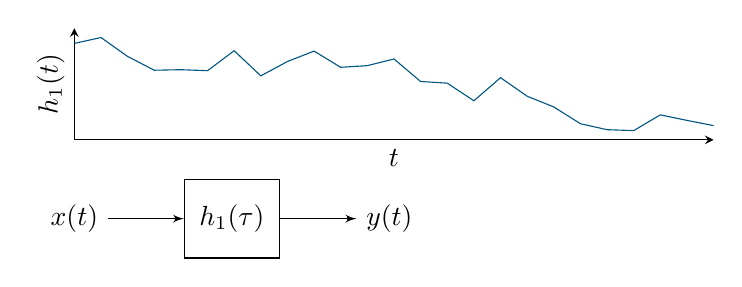
\begin{tikzpicture}[auto, node distance=2cm,>=latex']
  \begin{axis}[
      height=3cm,
      width=.8\textwidth,
    xlabel=$t$,
    ylabel=$h_1(t)$,
      samples=25,
      domain=0:2,
      ticks=none,
      axis x line=bottom,
      axis y line=left,
      enlarge y limits=true,
    ]
    \pgfmathsetseed{413}%
    \addplot[VCobalt] {4-pow(x,2) + 1*rand};
  \end{axis}
        \node [pinstyle] at (0,-1) (input)  {$x(t)$};
        \node [block, right of=input] (ch) {$h_1(\tau)$};
        \node [pinstyle,right of = ch] (output)  {$y(t)$};
        \draw[->] (input)--(ch);
        \draw[->] (ch)--(output);
    \end{tikzpicture}}
    \end{figure}
\end{column}
\begin{column}{6cm}
 \begin{figure}
    \centering
    \caption{Response at instant $t=t_o$}
\scalebox{.75}{
    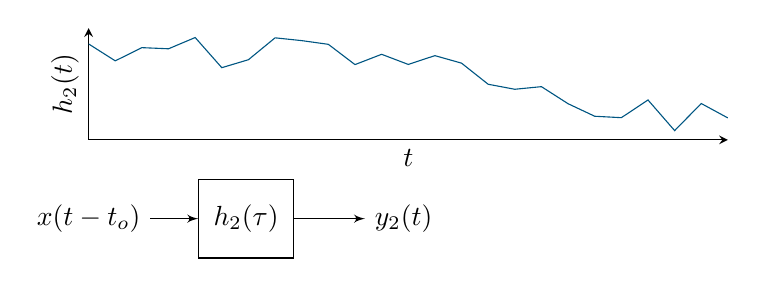
\begin{tikzpicture}[auto, node distance=2cm,>=latex']
  \begin{axis}[
      height=3cm,
      width=.8\textwidth,
    xlabel=$t$,
    ylabel=$h_2(t)$,
      samples=25,
      domain=0:2,
      ticks=none,
      axis x line=bottom,
      axis y line=left,
      enlarge y limits=true,
    ]
    \pgfmathsetseed{42}%
    \addplot[VCobalt] {4-pow(x,2) + 1*rand};
  \end{axis}
        \node [pinstyle]  at (0,-1) (input)  {$x(t-t_o)$};
        \node [block, right of=input] (ch) {$h_2(\tau)$};
        \node [pinstyle,right of = ch] (output)  {$y_2(t)$};
        \draw[->] (input)--(ch);
        \draw[->] (ch)--(output);
    \end{tikzpicture}}
    \end{figure}
\end{column}
\end{columns}

    \begin{itemize}    
     \item In general, 
     $$y_1(t)=\int_{-\infty}^{\infty}h_1(\tau)x(t-\tau)d\tau\;\neq\;y_2(t)=\int_{-\infty}^{\infty}h_2(\tau)x(t-t_o-\tau)d\tau$$
     \item If $h_1(t)=h_2(t)$ the channel is a Linear Time Invariant system
     $$y_2(t)=y_1(t-t_o)=h(t)*x(t-t_o)$$
     \end{itemize}
     \begin{definition}[Time Variant Channel]
      The input-output function $h(t_o,\tau)$ is 2-dimensional. $\tau$ is the \textbf{delay} variable of the integral (not a convolution) and $t_o$ is the \textbf{observation instant} variable representing the instant of the delta that generated the impulse response
     $$y(t-t_o)=\int_{-\infty}^{\infty}h(t_o,\tau)x(t-t_o-\tau)d\tau$$
     \end{definition}
     
     
 \begin{figure}
    \centering
    \caption{Probe the channel with a delta to obtain a time-varying impulse response}
    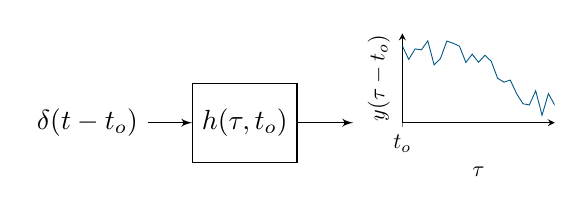
\begin{tikzpicture}[auto, node distance=2cm,scale=.8,>=latex']
        \node [pinstyle] (input)  {$\delta (t-t_o)$};
        \node [block, right of=input] (ch) {$h(\tau,t_o)$};
        \node [pinstyle,right of = ch, node distance=1.5cm] (output)  {};
        \draw[->] (input)--(ch);
        \draw[->] (ch)--(output);
        \node [coordinate,right of = output, node distance=.5cm] (graphcoord)  {};
        \begin{axis}[
        at={(graphcoord)},
      height=3cm,
      width=4cm,
    xlabel=$\tau$,
    ylabel=$y(\tau-t_o)$,
      samples=25,
      domain=0:2,
      xtick={0},
      xticklabels={$t_o$},
      ytick=\empty,
      axis x line=bottom,
      axis y line=left,
      enlarge y limits=true,
    ]
    \pgfmathsetseed{42}%
    \addplot[VCobalt] {4-pow(x,2) + 1*rand};
  \end{axis}
    \end{tikzpicture}
    \end{figure}
}

\frame[allowframebreaks]{\frametitle{Fading Statistics}
    \begin{figure}
     \centering
     \caption{Multipath Channel}
     \includesvg[width=.45\columnwidth]{multipath}
    \end{figure}
    \begin{itemize}
     \item Paths with AoD ($\theta_p(t)$), AoA ($\phi_p(t)$), delay ($\tau_p(t)$) and Doppler ($\nu_p(t)$)
     $$h_{i,j}(\tau,t_o)=\sum_{p=1}^{N_{path}}\sqrt{G_p}e^{-j2\pi\left[ \frac{d'_i\cos \theta_p(t)}{\lambda} + \frac{d'_j\cos \phi_p(t)}{\lambda} \textcolor{ARust}{ +\nu_p(t_o)  + f_c \tau_p(t_o) }+\angle_0\right]}\textcolor{ARust}{\delta(\tau-\tau_p(t_o))}$$
     \item If $f_c\tau_p\gg 1$, small change in $\tau_p$ causes a very large change in phase
     \item If $N_{path}$ is very large, apply CLT $\to$ \textbf{Fading channel}
    \end{itemize}
\pagebreak
$h(\tau,t_o)$ is a random ``vector'' (index $\tau$) \textbf{stochastic process} observed on $t_o$

\begin{definition}[Autocorrelation Function]
 $$A_{h}(\tau_1,\tau_2,t_1,t_2)=\Ex{}{h^*(\tau_1,t_1)h(\tau_2,t_2)}$$
\end{definition}

\begin{definition}[Wide Sense Stationary (WSS) stochastic process]
Autocorrelation depends only on $\Delta t=t_2-t_1\to$ $A_{h}(\tau_1,\tau_2,\Delta)$
\end{definition}
\begin{definition}[Uncorrelated Scattering]
No correlation of different delays $A_{h}(\tau_1,\tau_2,t_1,t_2)=\begin{cases}A_{h}(\tau,\Delta t)&\textnormal{if }\tau_1=\tau_2\\0 &\textnormal{if }\tau_1\neq\tau_2\end{cases}$
\end{definition}
\pagebreak
\begin{definition}[Scattering Function (WSSUS)]
$$S_h(\tau,\nu)=\mathcal{F.T.}_{\Delta t}\left[A_{h}(\tau,\Delta t)\right]=\int_{-\infty}^{\infty}A_{h}(\tau,\Delta t)e^{-j2\pi\nu \Delta t}d\Delta t$$ 
\end{definition}

\begin{itemize}
 \item For the multipath channel we can write
 $$S_h(\tau,\nu)=\sum_{p=1}^{N_{path}}\sqrt{G_p}\delta(\tau-\tau_p)\times\delta(\nu-\nu_p)$$
 \item 2D F.T. of the \textbf{periodogram} in signal spectrum analysis
\end{itemize}
}

\frame[allowframebreaks]{\frametitle{Frequency-Flat Scattering}
\begin{columns}
\begin{column}{6cm}
 \begin{figure}
    \centering
    \caption{Response 1}
    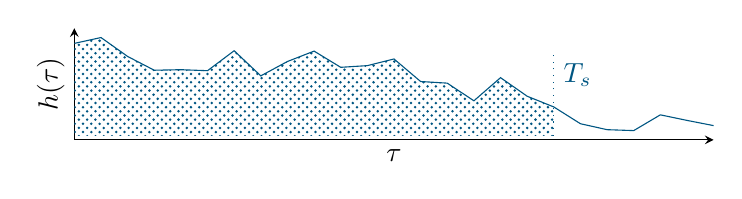
\begin{tikzpicture}[auto, node distance=2cm,>=latex']
  \begin{axis}[
      height=3cm,
      width=.8\textwidth,
    xlabel=$\tau$,
    ylabel=$h(\tau)$,
      samples=25,
      domain=0:2,
      ticks=none,
      axis x line=bottom,
      axis y line=left,
      enlarge y limits=true,
    ]
    \pgfmathsetseed{413}%
    \addplot[name path = A,VCobalt] {4-pow(x,2) + 1*rand};
    \path[name path=axis] (axis cs:0,0) -- (axis cs:2,0);
    % Fill area between paths
    \addplot [VCobalt,pattern color=VCobalt,pattern=crosshatch dots] fill between[of = A and axis, soft clip={domain=0:1.5}];
    \node[anchor=west,VCobalt] at (axis cs:1.5,3) {$T_s$};
    \draw[dotted,VCobalt] (axis cs:1.5,0) --  (axis cs:1.5,4) ;
  \end{axis}
    \end{tikzpicture}
    \end{figure}
\end{column}
\begin{column}{6cm}
 \begin{figure}
    \centering
    \caption{Response 2}
    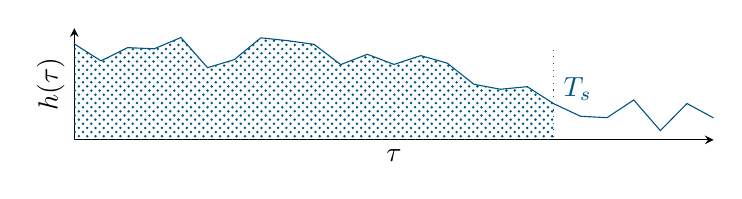
\begin{tikzpicture}[auto, node distance=2cm,>=latex']
  \begin{axis}[
      height=3cm,
      width=.8\textwidth,
    xlabel=$\tau$,
    ylabel=$h(\tau)$,
      samples=25,
      domain=0:2,
      ticks=none,
      axis x line=bottom,
      axis y line=left,
      enlarge y limits=true,
    ]
    \pgfmathsetseed{42}%
    \addplot[name path = A,VCobalt] {5-pow(x,2) + 1*rand};
    \path[name path=axis] (axis cs:0,0) -- (axis cs:2,0);
    % Fill area between paths
    \addplot [VCobalt,pattern color=VCobalt,pattern=crosshatch dots] fill between[of = A and axis, soft clip={domain=0:1.5}];
    \node[anchor=west,VCobalt] at (axis cs:1.5,3) {$T_s$};
    \draw[dotted,VCobalt] (axis cs:1.5,0) --  (axis cs:1.5,5) ;
  \end{axis}
    \end{tikzpicture}
    \end{figure}
\end{column}
\end{columns}
 \begin{itemize}
 \item Negligible energy outside 1 period $|h(\tau,\Delta t)|^2\simeq 0 \;\forall \tau\notin[0,T_s]$
 \item WSSUS \textbf{scalar} stochastic process $h(\tau,\Delta t)\simeq h_0(\Delta t)\delta(\tau)$
 \item Add the index $[n]$ to DEC gain
 $$y_j[n]=\textcolor{ARust}{h_{i,j}[n]}x_{i}[n]+z_{i}[n]\Rightarrow \y[n]=\textcolor{ARust}{\Hb[n]}\x[n]+\z[n]$$
 \item Question \textbf{What is the relation between $[n]$ and $\Delta t$?}
 \end{itemize}
 
 \pagebreak
\begin{columns}
\begin{column}{6cm}
 \begin{figure}
    \centering
    \caption{Uniform Scatterers}
    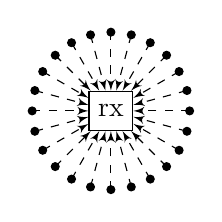
\begin{tikzpicture}[auto, node distance=2cm,>=latex']
    \node[block,draw, minimum size =.5cm] at (0,0) (rx) {rx};
    \foreach \x in {0,15,...,359}{
        \draw[fill=black] (\x:1) circle (.05cm);
        \draw[dashed,->] (\x:1) -- (rx);˙
        };
    \end{tikzpicture}
    \end{figure}
\end{column}
\begin{column}{6cm}
 \begin{figure}
    \centering
    \caption{Jakes Spectrum}
    \begin{tikzpicture}[auto, node distance=2cm,>=latex']
  \begin{axis}[
      height=3cm,
      width=\textwidth,
    xlabel=$\nu_p$,
    ylabel=$S(\nu_p)$,
      samples=100,
      xmin=-4,
      xmax=3,
      ymax=10,
      ticks=none,
      axis x line=bottom,
      axis y line=left,
      enlarge y limits=true,
    ]
    \addplot[samples=81,domain=-2:2,name path=f] {1/(2-abs(x))};
    \draw[thick,dashed] (axis cs:2, 0) -- node[anchor=west] {$f_D$} (axis cs:2, 10);
    \draw[thick,dashed] (axis cs:-2, 0) -- node[anchor=east] {$-f_D$} (axis cs:-2, 10);
  \end{axis}
    \end{tikzpicture}
    \end{figure}
\end{column}
\end{columns}
 \begin{itemize}
  \item Frequency Flat Rayleigh models by \textbf{Clarke and Jakes}
  \item Assume $\sqrt{G_p}$, $\tau_p$, and $\nu_p$ change slow, treat as constant
  \item $f_c\tau_p(\Delta t)\gg \nu_p\Delta t\to$ phase is $\approx U(0,2\pi)$
 \end{itemize}
    $$A(\Delta t)\approx \frac{P}{2}J_o(2\pi f_D \Delta t)\textnormal{ where } f_D=\frac{v_{\textnormal{speed}}}{\lambda}$$

 \begin{figure}
    \centering
    \caption{Correlation becomes zero at distance $\approx\lambda/2$}
    \begin{tikzpicture}[auto, node distance=2cm,>=latex']
  \begin{axis}[
      height=3cm,
      width=.5\textwidth,
        xlabel=$f_D\tau_p$,
        ylabel=$J_0(f_D\tau_p)$,
      samples=81,
      domain=0:20,
      ticks=none,
      axis x line=bottom,
      axis y line=left,
      enlarge y limits=true,
    ]
    \addplot[samples=81,VCobalt] gnuplot{besj0(x)};
    \draw[dotted] (axis cs:0,0) -- (axis cs:20,0);
    \draw[dashed] (axis cs:2.5,0) -- node[anchor=south west] {$\lambda/2$} (axis cs:2.5,-1);
  \end{axis}
    \end{tikzpicture}
    \end{figure}
    \vspace{-.1in}
\begin{itemize}
 \item Re-correlation is generally ignored except advanced analyses
\end{itemize}
 \begin{definition}[Coherence Time]
  Different definitions in different technologies, books or analyses...
   $$T_{coh}\stackrel{\textnormal{1st 0}}{\approx} \frac{\lambda/2}{v_{\textnormal{speed}}}$$
 \end{definition}
 }
\frame[allowframebreaks]{\frametitle{Fading Regimes}
 \begin{definition}[Transport Block]
  Sequence of $L_{s}=L_b/\eta$ consecutive modulation symbols \textbf{DECODED JOINTLY}. I.e. IP packet/MAC frame of $L_b$ bits using modulation size $\eta =\log_2(M)$. The transmitted signal is the sum of all finite-block signals.
  $$x[n]=\sum_{b=-\infty}^{\infty}x[\dot{n},b]\textnormal{ where } \dot{n}=n \mod L_{s} \in \{0,L_{s}-1\}$$
 \end{definition}
 \vspace{-.1in}
 \begin{definition}[Fast Fading]
  $T_{coh}\lesssim T_s$. In each block $L_{s}$ i.i.d. realizations of the stochastic process
    $$y[\dot{n},b]= h[\textcolor{ARust}{\dot{n}},b]x[\dot{n},b]+z[\dot{n},b],\;h[\dot{n},b]\sim \textnormal{i.i.d. }\forall \dot{n},b$$
  \end{definition}
  \pagebreak
  \begin{figure}
   \centering
   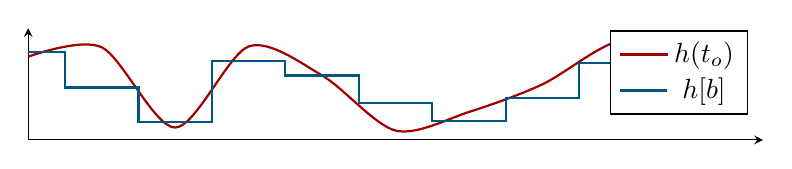
\begin{tikzpicture}
    \begin{axis}[ymax=1,xmin=0,xmax=10,height=3cm,width=.9\columnwidth,
      ticks=none,
      axis x line=bottom,
      axis y line=left,
      enlarge y limits=true,]
    \addplot[smooth,samples=20,domain=0:1,ARust,thick] coordinates{
        (0,0.8147)
        (1,0.9058)
        (2,0.1270)
        (3,0.9134)
        (4,0.6324)
        (5,0.0975)
        (6,0.2785)
        (7,0.5469)
        (8,0.9575)
        (9,0.9649)
    };
    \addplot[samples=20,domain=0:1,VCobalt,thick] coordinates{
        (0.0,0.8603)
        (0.5,0.8603)
        (0.5,0.5164)
        (1.5,0.5164)
        (1.5,0.18)
        (2.5,0.18)
        (2.5,0.7729)
        (3.5,0.7729)
        (3.5,0.6324)
        (4.5,0.6324)
        (4.5,0.3649)
        (5.5,0.3649)
        (5.5,0.1880)
        (6.5,0.1880)
        (6.5,0.4127)
        (7.5,0.4127)
        (7.5,0.7522)
        (8.5,0.7522)
        (8.5,0.9612)
        (9.5,0.9612)
    };
    \legend{$h(t_o)$,$h[b]$}
    \end{axis}
   \end{tikzpicture}
  \end{figure}

  \begin{definition}[Block Fading]
  $T_{coh}\approx L_{s}T_s$. Channel \textbf{approximated} by block-by-block i.i.d. model
  $$y[\dot{n},b]\textcolor{VCobalt}{\simeq h[b]}x[\dot{n},b]+z[\dot{n},b], h[b]\textcolor{VCobalt}{\approx \textnormal{i.i.d. }\forall b}$$
  \end{definition}
 \vspace{-.1in}
 \begin{definition}[Slow Fading]$T_{coh}\gg L_{s}T_s$. The channel is random but remains the same in all blocks
  $$y[\dot{n},b]=\textcolor{ARust}{h}x[\dot{n},b]+z[\dot{n},b], \textcolor{ARust}{h\textnormal{ same }\forall b}$$
  \end{definition}
}

\frame{\frametitle{MIMO Fading Channels}
    \begin{itemize}
     \item Matrix channel notation $\y[n]= \Hb[n]\x[n]+\z[n]$
     \item Fast/Block/Slow fading $\to$ correlation of $\Hb[\dot{n}_1,b_1]$ vs $\Hb[\dot{n}_2,b_2]$ 
     \item Spatial correlation $\to$ $\Sg_{\vstack{\Hb}}=\Ex{}{\vstack{\Hb}\vstack{\Hb}^H}\neq \I_{N_{t}N_{r}}$ 
     \item Normalization $\Ex{}{\|\Hb[n]\|^2}=\Ex{}{\vstack{\Hb}^H\vstack{\Hb}}=N_{t}N_{r}\to\sigma_h^2=1$
    \end{itemize}
    \begin{definition}[Instantaneous and Average SNR]
     $$\rho(\Hb[n])=\frac{P\|\Hb[n]\|^2}{N_{t}N_{r}\sigma_z^2}$$
     $$\overline{\rho}=\Ex{}{\rho(\Hb[n])}=\frac{P\Ex{}{\|\Hb[n]\|^2}}{N_{t}N_{r}\sigma_z^2}=\frac{P\sigma_h^2}{\sigma_z^2}$$
    \end{definition}
}

\frame[allowframebreaks]{\frametitle{SISO Fast Fading}
    \begin{itemize}
    \item Each decoded block experiences lots of fading realizations
        $$y[n]= h[n]x[n]+z[n]$$
    \item If $\mathscr{B}(\rho)=$ AWGN BER with SNR $\rho$
        $$\overline{\mathscr{B}(\rho)}=\Ex{h}{\mathscr{B}(\rho)}=\int f(\rho)\mathscr{B}(\rho)d\rho=\int f(|h|^2)\mathscr{B}\left(\frac{P|h|^2}{\sigma_z^2}\right)d|h|^2$$
    \item Example: BPSK with Rayleigh channel ($g_h=|h|^2$)
    $$\overline{\mathscr{B}(\rho)}=\int_0^\infty \frac{1}{\sigma_h^2} e^{-\frac{g_h}{\sigma_h^2}}\mathcal{Q}\left(\sqrt{2\overline{\rho}\frac{g_h}{\sigma^2_h}}\right)d g_h=\frac{1}{2}\left[1-\sqrt{\frac{\overline{\rho}}{\overline{\rho}+1}}\right]\stackrel{\textnormal{Taylor}}{\approx} O(\frac{1}{4\overline{\rho}})$$
    \end{itemize}
 
\begin{columns}
 \begin{column}{7cm}
  \begin{figure}
   \centering
   \caption{BPSK BER}
   \begin{tikzpicture}
    \begin{semilogyaxis}[ymax=1,ymin=1e-3,xmin=0,xmax=30,height=6cm,width=.99\columnwidth,      
      axis x line=bottom,
      axis y line=left,
      enlarge y limits=true,
      xlabel = $\overline{\rho}$ (dB),
      ylabel = BER]
      \addplot[VCobalt,domain=0:10,samples=100] gnuplot{2*erfc(sqrt(2*10^(x/10)))};
      \addplot[TZTeal,domain=0:10,samples=100] {.5(exp(-sqrt(2)*pow(10,x/10)))};
      \addplot[ARust,domain=0:30,samples=100] {.5(1-sqrt(pow(10,x/10)/(pow(10,x/10)+1)))};
      \addplot[KYJade,domain=0:30,samples=100] {2/(4*pow(10,x/10))};
      \draw[<->] (axis cs:7,0.001) -- node[anchor=south] {$20dB$} (axis cs:27,.001);
    \legend{AWGN,Chernoff,Rayleigh,Taylor}
    \end{semilogyaxis}
   \end{tikzpicture}
  \end{figure}
 \end{column}
 \begin{column}{6cm}
  \begin{itemize}
   \item Chernoff Bound
   $$Q(x)\lesssim \frac{1}{2}e^{-\frac{x^2}{2}}$$   
   \item AWGN BER $\mathscr{B}(\overline{\rho})\approx e^{-\overline{\rho}}$\\ \ \\
   \item Rayleigh BER $\overline{\mathscr{B}(\rho)}\approx \overline{\rho}^{-1}$\\ \ \\
   \item Huge SNR requirement difference   
   \item Same other modulations changing $\mathscr{B}(\rho)$
  \end{itemize}
 \end{column}
\end{columns}

\begin{definition}[Diversity]
Transmission of multiple copies of the same bit in independent channels 
\end{definition}
  \begin{figure}
   \centering
   \caption{Diversity BER$\approx \rho^{-D}$}
   \begin{tikzpicture}
    \begin{semilogyaxis}[ymax=1,ymin=1e-3,xmin=0,xmax=30,height=5cm,width=.7\columnwidth,      
      axis x line=bottom,
      axis y line=left,
      enlarge y limits=true,
      xlabel = $\overline{\rho}$ (dB),
      ylabel = BER]
%       \addplot[ARust,domain=0:30,samples=100] {.5(1-sqrt(pow(10,x/10)/(pow(10,x/10)+1)))};
      \addplot[ARust,domain=0:30,samples=100] {2/(4*pow(10,x/10))};
      \addlegendentry{$D=1$}
      \addplot[TAMustard,domain=0:30,samples=100] {2*pow(2/(4*pow(10,x/10)),2)};
      \addlegendentry{$D=2$}
      \addplot[KYJade,domain=0:30,samples=100] {3*pow(2/(4*pow(10,x/10)),3)};
      \addlegendentry{$D=3$}
      \addplot[TZTeal,domain=0:30,samples=100] {4*pow(2/(4*pow(10,x/10)),4)};
      \addlegendentry{$D=4$}
      \addplot[VCobalt,domain=0:10,samples=100] gnuplot{2*erfc(sqrt(2*10^(x/10)))};
      \addlegendentry{AWGN}
%       \addplot[TZTeal,domain=0:10,samples=100] {.5(exp(-sqrt(2)*pow(10,x/10)))};
%       \addlegendentry{Chernoff}
%     \legend{AWGN,Chernoff,Rayleigh,Taylor}
    \end{semilogyaxis}
   \end{tikzpicture}
  \end{figure}
  
\begin{definition}[Outage Probability vs threshold $\xi$]
$$P_o=P(\rho(h)<\xi)=P(|h|^2<\xi)=F_{|h|^2}(\xi)$$
\end{definition} 
\begin{itemize}
 \item We can set any BER threshold $\beta$ and evaluate $\xi=\mathscr{B}^{-1}(\beta)$ 
 \item Approximation $\mathscr{B}(\rho)\approx\begin{cases}
                                          0&\textnormal{ if }\rho>\xi\\
                                          1&\textnormal{ if }\rho\leq\xi\\
                                         \end{cases} \Rightarrow \overline{\mathscr{B}(\rho)}\approx P_o \approx \overline{\rho}^{-D}$
\end{itemize}
\begin{columns}
 \begin{column}{6cm}
\begin{figure}
   \centering
   \caption{Rayleigh 10\%-iles for BER=$10^{-3}$}
   \scalebox{.7}{
   \begin{tikzpicture}
    \begin{semilogyaxis}[ymax=1,ymin=1e-3,xmin=0,xmax=20,height=4cm,width=.99\columnwidth,      
      axis x line=bottom,
      axis y line=left,
      enlarge y limits=true,
      xlabel = $\overline{\rho}$ (dB),
      ylabel = BER]
      \addplot[VCobalt,domain=0:20,samples=100] gnuplot{2*erfc(sqrt(2*0.0513*10^(x/10)))};
      \addplot[VCobalt,domain=0:20,samples=100] gnuplot{2*erfc(sqrt(2*0.1054*10^(x/10)))};
      \addplot[VCobalt,domain=0:20,samples=100] gnuplot{2*erfc(sqrt(2*.2231*10^(x/10)))};
      \addplot[VCobalt,domain=0:20,samples=100] gnuplot{2*erfc(sqrt(2*0.3567*10^(x/10)))};
      \addplot[VCobalt,domain=0:20,samples=100] gnuplot{2*erfc(sqrt(2*0.5108*10^(x/10)))};
      \addplot[VCobalt,domain=0:20,samples=100] gnuplot{2*erfc(sqrt(2*0.6931*10^(x/10)))};
      \addplot[VCobalt,domain=0:20,samples=100] gnuplot{2*erfc(sqrt(2*0.9163*10^(x/10)))};
      \addplot[VCobalt,domain=0:20,samples=100] gnuplot{2*erfc(sqrt(2*1.2040*10^(x/10)))};
      \addplot[VCobalt,domain=0:20,samples=100] gnuplot{2*erfc(sqrt(2*1.6094*10^(x/10)))};
      \addplot[VCobalt,domain=0:20,samples=100] gnuplot{2*erfc(sqrt(2*2.3026*10^(x/10)))};
      \addplot[black,dashed,mark=*,mark options={solid}] coordinates{
  (17.7123,1e-3)
  (14.5861,1e-3)
  (11.3270,1e-3)
   (9.2901,1e-3)
   (7.7301,1e-3)
   (6.4046,1e-3)
   (5.1925,1e-3)
   (4.0067,1e-3)
   (2.7461,1e-3)
   (1.1907,1e-3)
    };
    \node[anchor=south] at(axis cs:17.7123,1e-3) {$5$\%};
    \node[anchor=south] at(axis cs:14.5861,1e-3) {$10$\%};
    \node[anchor=south] at(axis cs:1.1907,1e-3) {$90$\%};
    \end{semilogyaxis}
   \end{tikzpicture}}
  \end{figure}
 \end{column}
 \begin{column}{6cm}
\begin{figure}
   \centering
   \caption{Rayleigh 10\%-iles}
   \scalebox{.7}{
   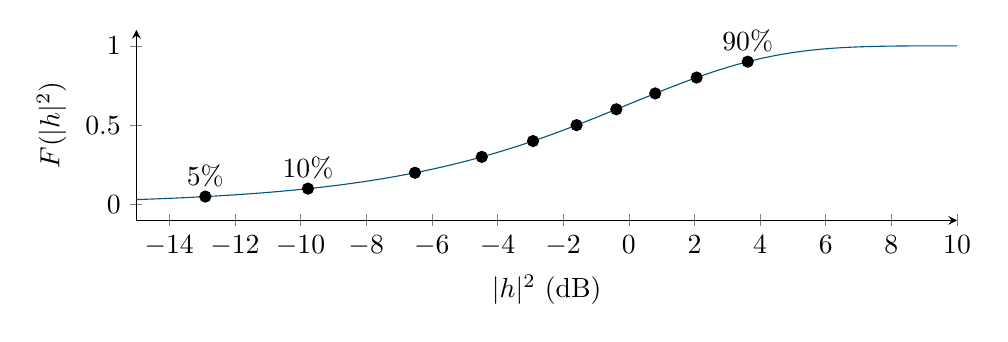
\begin{tikzpicture}
    \begin{axis}[ymax=1,ymin=0,xmin=-15,xmax=10,height=4cm,width=.99\columnwidth,      
      axis x line=bottom,
      axis y line=left,
      enlarge y limits=true,
      xlabel = $|h|^2$ (dB),
      ylabel = $F(|h|^2)$
      ]
      \addplot[VCobalt,domain=-15:15,samples=100] {1-exp(-pow(10,x/10))};
      \addplot[only marks,mark=*,mark options={solid}] coordinates{
   (-12.8994,.05)
   (-9.7732,.1)
   (-6.5142,.2)
   (-4.4773,.3)
   (-2.9173,.4)
   (-1.5917,.5)
   (-0.3797,.6)
    (0.8062,.7)
    (2.0667,.8)
    (3.6222,.9)
    };
    \node[anchor=south] at(axis cs:-12.8994,.05) {$5$\%};
    \node[anchor=south] at(axis cs:-9.7732,.1) {$10$\%};
    \node[anchor=south] at(axis cs:3.6222,.9) {$90$\%};
    \end{axis}
   \end{tikzpicture}}
  \end{figure}
 \end{column}
\end{columns}
  
\begin{definition}[Diversity Gain]
 Outage definition $\displaystyle D \triangleq \lim_{\overline{\rho}\to\infty} \frac{-\log P_o}{\log \overline{\rho}}$ vs BER definition $\displaystyle D \triangleq \lim_{\overline{\rho}\to\infty} \frac{-\log BER}{\log \overline{\rho}}$
\end{definition}

  \begin{itemize}
    \item Example: $\frac{1}{2}$ Repetition Code
    $$\left(\begin{array}{c}
                y[n]\\
                y[n+1]
            \end{array}\right)
            =
      \left(\begin{array}{c}
                h[n]\\
                h[n+1]
            \end{array}\right)
            x[ \lfloor n/2\rfloor]
            +
            \left(\begin{array}{c}
                z[n]\\
                z[n+1]
            \end{array}\right)$$
    \item Majority Decoding
    $$BER=\left(D(4\overline{\rho})^{-1} \right)^D\sum_{k=0}^{D-1}{D-1+k \choose k}(1-\left(D(4\overline{\rho})^{-1} \right)^{k})\approx \overline{\rho}^{-D}$$
    \item MRC linear processing
    \begin{equation*}
     \begin{split}
      r&=\frac{h^*[n]y[n]+h^*[n+1]xy[n+1]}{\sqrt{|h[n]|^2+|h[n+1]|^2}}\\
       &=\underset{\sqrt{G}}{\underbrace{\frac{(|h[n]|^2+|h[n+1]|^2)}{\sqrt{|h[n]|^2+|h[n+1]|^2}}}}x+z'
     \end{split}
    \end{equation*}
    \begin{definition}[Chi Squared Distribution]
    \begin{equation*}
     \begin{split}
      G=\sum_{k=0}^{D-1}|h[n+k]|^2\sim \chi^2(2D),\;f(G)=\frac{G^{D-1}e^{-G/2}}{2^{D}\Gamma(D)} \Rightarrow BER \approx \overline{\rho}^{-D}
     \end{split}
    \end{equation*}
    \end{definition}   
\end{itemize}
}

\frame{\frametitle{SISO Block/Slow Fading}
\begin{itemize}
    \item Each block/full system experiences \textbf{a single fading realization}
        $$y[\dot{n},b]= h[b]x[\dot{n},b]+z[\dot{n},b]$$
    \item Instantaneous SNR $\rho$ and AWGN BER $\mathscr{B}(\rho)$ (not averaged)\\ \ \\
    \item Outage probability $P_o$ $\approx$ TB Error Rate (BLER)\\ \ \\
    \item \textbf{Diversity} important for different reasons
    \begin{itemize}
        \item In Fast Fading, improve BER vs $\overline{\rho}$
        \item In Slow Fading, improve $P_o$ vs $\overline{\rho}$
        \item In Block Fading, $L_{s}\approx T_{coh}$ vs decoding delay
\end{itemize}
\end{itemize}
}
\frame[allowframebreaks]{\frametitle{Information in Fading Channels}

\begin{proof}[Inside of Shannon's Proof]
\begin{itemize}
 \item Channel used multiple times  $\{\x[n]\}_{n=0}^{L_{s}}$\\ \ \\
%     \begin{itemize}
%     \item Random constellation $\mathcal{C}$ with $R$ items, each $\x[n]\in\mathcal{C}$ p.d.f. $f(x)$
%     \end{itemize}
 \item {Chain rule} of M.I.  $\qquad \Inf{\{\x[n]\}_{n=0}^{L_{s}}}{\{\y[n]\}_{n=0}^{L_{s}}}\stackrel{}{=}\Inf{\x[0]}{\{\y[n]\}_{n=0}^{L_{s}}}+\CInf{\{\x[n]\}_{\textcolor{ARust}{n=1}}^{L_{s}}}{\{\y[n]\}_{n=0}^{L_{s}}}{\textcolor{ARust}{\x[0]}}\dots$\\ \ \\
 \item $C$ defined $\max R$ s.t. \textbf{probability of error is as low as desired}.
    \begin{itemize}
    \item $R\leq C$ if and \textbf{only if} $\displaystyle\lim_{L_{s}\to\infty} P(\hat{x}\neq x) = 0 $\\ \ \\
    \end{itemize}
 \item Instantaneous M.I. is a function of channel $\CInf{\x}{\y}{\Hb}=\mathcal{I}(\Hb)$\\ \ \\
 \item \textcolor{ARust}{Formally, the Shannon capacity of fading channels is zero!}

\end{itemize} 
\end{proof}

\pagebreak

\begin{definition}[Ergodic Capacity]
In \textbf{Fast Fading}, as $L_{s}\to\infty$ the frame $\{\x[n]\}_{n=0}^{L_{s}}$ sees \textit{infinite realizations} of the random channel. The M.I. $\mathcal{I}(\Hb[n])$ is averaged over $f(\Hb)$
\begin{itemize}
     \item With CSIR the transmitter uses same $f(\x)\; \forall \Hb$
        $$C=\sup_{\x}\Ex{\Hb}{ \CInf{\x[n]}{\y[n]}{\Hb[n]}}$$
     \item With CSIT the transmitter modifies $f(\x|\Hb)$ for each value of $\Hb$
        $$C=\Ex{\Hb}{ \sup_{\x} \CInf{\x[n]}{\y[n]}{\Hb[n]}}$$
    \end{itemize}
\end{definition}
\begin{itemize}
 \item By Jensen's Inequality $\Ex{\rho}{\log(1+\rho)}\leq\log(1+\Ex{\rho}{\rho})$\\ \ \\
 \item The Ergodic Capacity is \textbf{achievable} using long $L_{s}$ and joint coding
 \begin{itemize}
    \item One of the great advantages of OFDM with i.i.d. subcarriers
        $$\lim_{K\to\infty} \sum_{k=0}^{K-1}\log\det\left(\I+\frac{P_k}{\sigma_z}\Hb[k]\Hb^H[k]\right)=\Ex{\Hb}{\sup \CInf{\x}{\y}{\Hb}}$$
    \item With CSIT $P_k$ waterfilling over time-domain or OFDM subcarriers\\ \ \\
 \end{itemize}
 \item Inefficient codes such as Repetition Coding are not enough\\ \ \\
 \item Advanced FEC codes based on MAP
 \begin{itemize}
    \item Turbo Codes (2 Convolutionals)
    \item Low Density Parity Check (LDPC)
 \end{itemize}
 \item Polar Codes in 5G
\end{itemize}
\pagebreak

\begin{definition}[Outage Capacity]
In \textbf{Slow Fading} only a single value of $\Hb$ observed per frame
    \begin{itemize}
     \item New definition of \textbf{Outage versus rate:}
     \begin{itemize}
        \item \underline{First} $R$ is chosen, \underline{after that} $\Hb$ is observed
        \item C.D.F. of $\CInf{\{\x[n]\}_{n=1}^{N}}{\{\y[n]\}_{n=1}^{N}}{\Hb}=\mathcal{I}_{n=1}^{N}(\Hb)\;\to\; P_o=F_{\mathcal{I}}(R)$
    \end{itemize}
     \item Capacity with outage requirement $P_o$
        $$C_{out}\triangleq \sup \{R \textnormal{ such that }  F_{\mathcal{I}}(R)\leq P_o\}$$
    \end{itemize}
\end{definition}
    \begin{itemize}
     \item Example: Rayleigh single antenna AWGN channel
        $$F_{\mathcal{I}}(R)=F_{|h|^2}\left(\textcolor{ARust}{\frac{\sigma_z^2(2^{R}-1)}{P}}\right)=1-e^{-\frac{1}{\sigma_h^2}\textcolor{ARust}{\frac{\sigma_z^2(2^{R}-1)}{P}}}=1-e^{-\frac{\xi(R)}{\overline{\rho}}}$$
        
    \item After $\Hb$ is revealed, Outage Capacity achievable as in AWGN\\ \ \\
    \item For the case of \textbf{Block Fading} there are different technologies where both Ergodic and Outage Capacity have a significance:\\ \ \\
    \begin{itemize}
        \item If the data packet is sufficiently long compared to $T_{coh}$, many blocks are transmitted and ergodic rate is observed.\begin{figure}
   \centering
   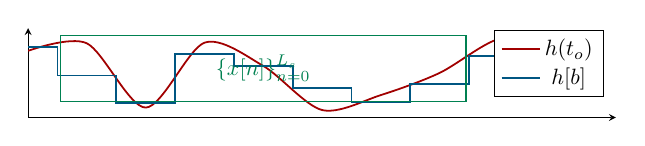
\begin{tikzpicture}[scale=.8]
    \begin{axis}[ymax=1,xmin=0,xmax=10,height=3cm,width=.9\columnwidth,
      ticks=none,
      axis x line=bottom,
      axis y line=left,
      enlarge y limits=true,]
    \addplot[smooth,samples=20,domain=0:1,ARust,thick] coordinates{
        (0,0.8147)
        (1,0.9058)
        (2,0.1270)
        (3,0.9134)
        (4,0.6324)
        (5,0.0975)
        (6,0.2785)
        (7,0.5469)
        (8,0.9575)
        (9,0.9649)
    };
    \addplot[samples=20,domain=0:1,VCobalt,thick] coordinates{
        (0.0,0.8603)
        (0.5,0.8603)
        (0.5,0.5164)
        (1.5,0.5164)
        (1.5,0.18)
        (2.5,0.18)
        (2.5,0.7729)
        (3.5,0.7729)
        (3.5,0.6324)
        (4.5,0.6324)
        (4.5,0.3649)
        (5.5,0.3649)
        (5.5,0.1880)
        (6.5,0.1880)
        (6.5,0.4127)
        (7.5,0.4127)
        (7.5,0.7522)
        (8.5,0.7522)
        (8.5,0.9612)
        (9.5,0.9612)
    };
    \legend{$h(t_o)$,$h[b]$}
    \draw[KYJade,thick] (0.55,0.2) rectangle (7.45,1);
    \node[KYJade] at (4,.6) {$\{x[n]\}_{n=0}^{L_{s}}$};
    \end{axis}
   \end{tikzpicture}
  \end{figure}
        \item If the data packet is very short compared to $T_{coh}$, only one frame is transmitted and $P_o\approx$ packet loss.
         \begin{figure}
   \centering
   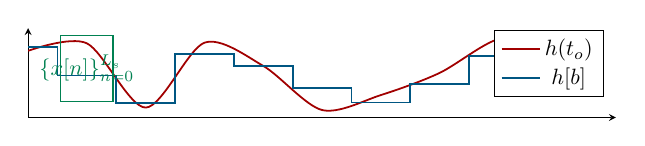
\begin{tikzpicture}[scale=.8]
    \begin{axis}[ymax=1,xmin=0,xmax=10,height=3cm,width=.9\columnwidth,
      ticks=none,
      axis x line=bottom,
      axis y line=left,
      enlarge y limits=true,]
    \addplot[smooth,samples=20,domain=0:1,ARust,thick] coordinates{
        (0,0.8147)
        (1,0.9058)
        (2,0.1270)
        (3,0.9134)
        (4,0.6324)
        (5,0.0975)
        (6,0.2785)
        (7,0.5469)
        (8,0.9575)
        (9,0.9649)
    };
    \addplot[samples=20,domain=0:1,VCobalt,thick] coordinates{
        (0.0,0.8603)
        (0.5,0.8603)
        (0.5,0.5164)
        (1.5,0.5164)
        (1.5,0.18)
        (2.5,0.18)
        (2.5,0.7729)
        (3.5,0.7729)
        (3.5,0.6324)
        (4.5,0.6324)
        (4.5,0.3649)
        (5.5,0.3649)
        (5.5,0.1880)
        (6.5,0.1880)
        (6.5,0.4127)
        (7.5,0.4127)
        (7.5,0.7522)
        (8.5,0.7522)
        (8.5,0.9612)
        (9.5,0.9612)
    };
    \legend{$h(t_o)$,$h[b]$}
    \draw[KYJade,thick] (0.55,0.2) rectangle (1.45,1);
    \node[KYJade] at (1,.6) {$\{x[n]\}_{n=0}^{L_{s}}$};
    \end{axis}
   \end{tikzpicture}
  \end{figure}
    \end{itemize}
    \end{itemize}
}


\frame[allowframebreaks]{\frametitle{Methods to achieve Diversity}
\begin{figure}
 \centering
 \caption{Time Diversity}
 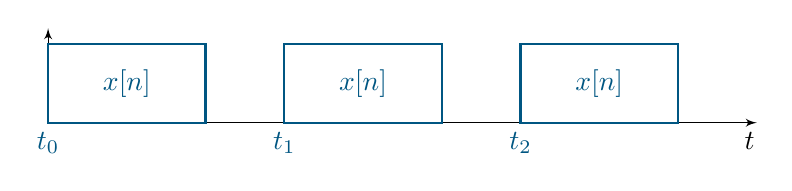
\begin{tikzpicture}[auto, node distance=2cm,>=latex']
  \draw[->] (0,0) -- node[pos=0.99,anchor=north] {$t$} (9,0);
  \draw[->] (0,0) -- (0,1.2);
  \foreach \x in {0,1,...,2}{
    \draw[VCobalt,thick] (3*\x,0) rectangle +(2,1);
    \node[VCobalt] at (3*\x+1,.5) {$x[n]$};
    \node[VCobalt,anchor=north] at (3*\x,0) {$t_{\x}$};
  };
 \end{tikzpicture}
\end{figure}

 \begin{itemize}
 \item $D$ repetitions over time (advanced FEC possible)
 \item Requires fast fading or block fading
 \item Increases delay (especially block fading)
 \item Modulation rate is divided by a factor $\frac{1}{D}$\\ \ \\
 \end{itemize}
 
\begin{figure}
 \centering
 \caption{Frequency Diversity}
 \begin{tikzpicture}[auto, node distance=2cm,>=latex']
  \draw[->] (0,0) -- node[pos=0.99,anchor=north] {$f$} (9,0);
  \draw[->] (0,0) -- (0,1.4);
  \foreach \x in {0,1,...,2}{
    \draw[VCobalt,thick,->] (3*\x+2,0) -- +(0,1);
    \node[VCobalt,anchor=south] at (3*\x+2,1) {$x[k]$};
    \node[VCobalt,anchor=north] at (3*\x+2,0) {$f_{\x}$};
  };
 \end{tikzpicture}
\end{figure}

 \begin{itemize}
\item $D$ repetitions over frequency (OFDM, CDMA... + FEC)
 \item Requires frequency selective channel with large bandwidth
 \item Spectral efficiency divided by a factor $\frac{1}{D}$\\ \ \\
 \end{itemize}

\begin{figure}
 \centering
 \caption{Code Diversity}
    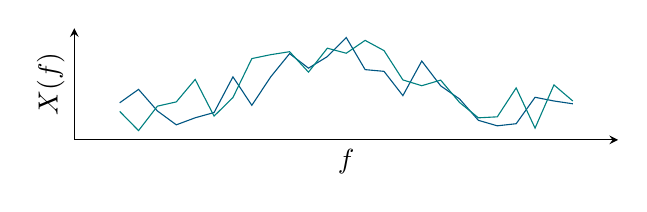
\begin{tikzpicture}[auto, node distance=2cm,>=latex']
        \begin{axis}[
            height=3cm,
            width=.7\textwidth,
            xlabel=$f$,
            ylabel=$X(f)$,
            samples=25,            
            domain=-1.2:1.2,
            xmin=-1.2,
            xmax=1.2,
            ticks=none,
            axis x line=bottom,
            axis y line=left,
            enlarge y limits=true,
            ]
            \pgfmathsetseed{413}%
            \addplot[domain=-1:1,VCobalt,samples=25] { 1-abs(x)+.5*rand};
            \pgfmathsetseed{42}%
            \addplot[domain=-1:1,TZTeal,samples=25] { 1-abs(x)+ .5*rand};
        \end{axis}
    \end{tikzpicture}
\end{figure}

 \begin{itemize}
 \item $D$ repetitions using different Spread Spectrum codes
 \item Frequency selective channel with large bandwidth
 \item Spectral efficiency divided by a factor $\frac{1}{D}$\\ \ \\
 \end{itemize}
 
 \textbf{Spatial Diversity (Antennas)}
 
 \begin{columns}
 \begin{column}{6cm}    
\begin{figure}
 \centering
 \caption{SIMO Channel}
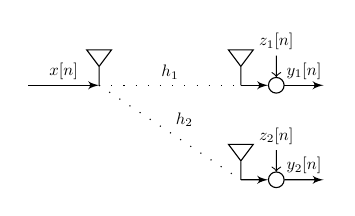
\begin{tikzpicture}[auto, node distance=2cm,>=latex', scale=0.6, every node/.style={scale=0.6}]
    \node [input, name=input] {};
    \node [input, right of=input, node distance=1.5cm, name=txant] {};
    \draw [draw] (txant) \antenna;
    \draw [draw,->,align=center] (input) -- node {$x[n]$} (txant);
    \node [input, right of=txant, node distance=3cm, name=rxant1] {};
    \node [input, below of=rxant1, node distance=2cm, name=rxant2] {};
    \draw [draw,loosely dotted,-,align=center] (txant)  -- node {$h_1$} (rxant1);
    \draw [draw,loosely dotted,-,align=center] (txant)  -- node {$h_2$} (rxant2);
    \draw [draw] (rxant1) \antenna;
    \draw [draw] (rxant2) \antenna;
    \node [sum, right of=rxant1, node distance=.75cm, pin={[pinstyle]above:$z_1[n]$}] (sum1) {};
    \node [sum, right of=rxant2, node distance=.75cm, pin={[pinstyle]above:$z_2[n]$}] (sum2) {};
    \draw [draw,->,align=center] (rxant1) -- (sum1);
    \draw [draw,->,align=center] (rxant2) -- (sum2);
    \node [input, right of=sum1, name=output1] {};
    \node [input, right of=sum2, name=output2] {};
    \draw [draw,->,align=center] (sum1) -- node {$y_1[n]$} (output1);
    \draw [draw,->,align=center] (sum2) -- node {$y_2[n]$} (output2);         
\end{tikzpicture}
\end{figure}
\begin{itemize}
 \item MRC with CSIR
    $$\rho=\frac{(|h_1|^2+|h_2|^2+\dots)P}{\sigma_z^2}\sim \frac{P}{\sigma_z^2\sqrt{2}}\chi^2(2N_{r})$$
 \item Array Gain $\overline{\rho}=\frac{PN_{r}}{\sigma_z^2}$
 \item Diversity $P_o\propto \overline{\rho}^{-N_{r}}$
 \end{itemize}
 \end{column}
 \begin{column}{6cm}
\begin{figure}
 \centering
 \caption{MISO Channel}
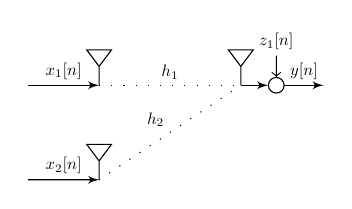
\begin{tikzpicture}[auto, node distance=2cm,>=latex', scale=0.6, every node/.style={scale=0.6}]
    \node [input, name=input1] {};
    \node [input, below of=input1, node distance=2cm, name=input2] {};
    \node [input, right of=input1, node distance=1.5cm, name=txant1] {};
    \node [input, right of=input2, node distance=1.5cm, name=txant2] {};
    \draw [draw] (txant1) \antenna;
    \draw [draw] (txant2) \antenna;
    \draw [draw,->,align=center] (input1) -- node {$x_1[n]$} (txant1);
    \draw [draw,->,align=center] (input2) -- node {$x_2[n]$} (txant2);
    \node [input, right of=txant1, node distance=3cm, name=rxant1] {};
    \draw [draw,loosely dotted,-,align=center] (txant1)  -- node {$h_1$} (rxant1);
    \draw [draw,loosely dotted,-,align=center] (txant2)  -- node {$h_2$} (rxant1);
    \draw [draw] (rxant1) \antenna;
    \node [sum, right of=rxant1, node distance=.75cm, pin={[pinstyle]above:$z_1[n]$}] (sum1) {};
    \draw [draw,->,align=center] (rxant1) -- (sum1);
    \node [input, right of=sum1, name=output1] {};
    \draw [draw,->,align=center] (sum1) -- node {$y[n]$} (output1);         
\end{tikzpicture}
\end{figure}
\begin{itemize}
 \item CSIR $\to$ 
    $$\rho=\frac{|\overset{Gaussian}{\overbrace{h_1+h_2+\dots}}|^2P}{N_{t}\sigma_z^2}\sim \frac{\cancel{N_{t}}P}{\cancel{N_{t}}\sigma_z^2}\textnormal{Exp}(1)$$
 \item CSIT $\to$ as in MRC SIMO
 \end{itemize}
 \end{column}
\end{columns}
}


\frame[allowframebreaks]{\frametitle{Diversity-Multiplexing Trade-Off}

\begin{itemize}
 \item Capacity $\to$ Eigenchannels $\to$ Spatial Multiplexing\\ \ \\
 \item Ergodic/Outage Capacity $\to$ Fast/Slow Fading $\to$ Diversity\\ \ \\
 \item What is best to do in random \textbf{MIMO} channels?\\ \ \\
 \item Example: Consider Rayleigh $\Hb\in\mathbb{C}^{N_{t},N_{r}}$
    \begin{itemize}
        \item Maximum diversity gain $D=\Ex{}{\|\Hb\|^2}=N_{r}N_{t}$, \textcolor{ARust}{but 1 symbol}\\ \ \\
        \item Maximum DoF $P(\mathrm{rank}(\Hb)=\min(N_{r},N_{t}))\approx 1$, \textcolor{ARust}{but $D=1$}\\ \ \\
    \end{itemize}
\end{itemize}

\begin{definition}[Diversity Gain]
 $$ D \triangleq \lim_{\overline{\rho}\to\infty} \frac{-\log P_o}{\log \overline{\rho}}\approx \textnormal{BER}=\overline{\rho}^{-D}$$
\end{definition}
\begin{definition}[Multiplexing Gain]
$$M=\lim_{\overline{\rho}\to\infty}\frac{R}{\log(\overline{\rho})}\Rightarrow M\leq \textnormal{DoF}$$
\end{definition}
\pagebreak
\begin{theorem}[Diversity-Multiplexing Trade-off]
The collection of values of rate multiplexing ($M$) that can be achieved with outage robustness corresponding to diversity $D(M)$
$$D(M)=\lim_{\overline{\rho}\to\infty}\frac{-\log\left[P\left(\mathcal{I}>M\log(\overline{\rho})\right)\right]}{\log(\overline{\rho})}\to \xi\propto \overline{\rho}^{M}$$
 In a Rayleigh fading channel $\Hb\in\mathbb{C}^{N_{t},N_{r}}$ we can achieve
 $$\textnormal{DMT-Rayleigh}=\begin{cases}
                            M\in\{0,\dots \min(N_{t},N_{r})\}\\
                            D(M)\leq (N_{t}-M)(N_{r}-M)
                           \end{cases}$$
\end{theorem}
 \begin{itemize}
  \item Example: DMT of a SISO channel $D(M)=1-M$
 \begin{itemize}
  \item Fix $\xi(R)$ constant, $P_o$ decreases with $\overline{\rho}^{-1}$
  \item Increase $\xi(R)$ as $\overline{\rho}^{1}$, $P_o$ remains constant
\end{itemize}
\end{itemize}

\begin{figure}
 \centering
 \caption{DMT}
    \begin{tikzpicture}[auto, node distance=2cm,>=latex']
        \begin{axis}[
            height=5cm,
            width=.7\textwidth,
            samples=25,            
            domain=0:4.2,
            xmin=0,
            xmax=4.2,
            ymin=0,
            ymax=16.2,
            axis x line=bottom,
            axis y line=left,
            xtick = {0,.6,1.53,2.25,3,4},
            xticklabels= {{$0$},{$1$},{$2$},{$\dots$},{$\min(N_{t},N_{r})-1$},{$\min(N_{t},N_{r})$}},
            ytick = {.25,2.07,4.25,6.26,16},
            yticklabels= {{$1$},{$4$},{$\vdots$},{$(N_{t}-1)(N_{r}-1)$},{$N_{t}N_{r}$}},
            xticklabel style={rotate=15},
            ]
            \addplot[domain=0:1,dotted,gray,samples=100] { 16-16*x};
            \addplot[domain=0:2,dotted,gray,samples=100] { 9-4.5*x};
            \addplot[domain=0:3,dotted,gray,samples=100] { 4-1.25*x};
            \addplot[domain=0:4,dotted,gray,samples=100] { 1-.25*x};
            \addplot[domain=0:4,dashed,VCobalt]coordinates{
   (0,16)
   (.6,6.26)
   (1.53,2.07)
   (3,.25)
   (4,0)
    };
        \end{axis}
    \end{tikzpicture}
\end{figure}
}


\frame{\frametitle{Intuition of DMT}

\begin{columns}
\begin{column}{6cm}
\begin{itemize}
\item Choose $M$ largest $|h_{i,j}|^2$
\item \textbf{Different column and row}
\item $(N_{r}-1)(N_{t}-1)$ choices
\end{itemize}

  $$\Hb=\left(\begin{array}{cccc}
              \markOverlay{vert3i}h_{1,1}&\markOverlay{vert1i}h_{1,2}&\markOverlay{vert2i}h_{1,3}\\
             \markOverlay{hor1i}h_{2,1}&\markOverlay{ch1}h_{2,2}&h_{2,3}\markOverlay{hor1f}\\
             \markOverlay{hor2i}h_{3,1}&h_{3,2}&h_{3,3}\markOverlay{hor2f}\\
              \markOverlay{hor3i}h_{4,1}\markOverlay{vert3f}&h_{4,2}\markOverlay{vert1f}&h_{4,3}\markOverlay{vert2f}\markOverlay{hor3f}\\
             \end{array}\right)$$
 \onslide<1->{
    \drawOverlayCircle[thick,KYJade]{$(ch1)+(.5em,.4em)$}{1em}{}
}
\onslide<2->{
  \drawOverlayLine[thick, KYJade ]{$(vert1i)+(.5em,1em)$}{$(vert1f)+(-.5em,-.5em)$}{}
  \drawOverlayLine[thick, KYJade ]{$(hor1i)+(0,.5em)$}{$(hor1f)+(0,.5em)$}{}
  \drawOverlayCircle[thick,ARust]{$(hor2f)+(-.7em,.4em)$}{1em}{}
}
\onslide<3->{
  \drawOverlayLine[thick, ARust ]{$(vert2i)+(.5em,1em)$}{$(vert2f)+(-.5em,-.5em)$}{}
  \drawOverlayLine[thick, ARust ]{$(hor2i)+(0,.5em)$}{$(hor2f)+(0,.5em)$}{}
  \drawOverlayCircle[thick,FFucsia]{$(hor3i)+(.5em,.4em)$}{1em}{}
}
\onslide<4->{
  \drawOverlayLine[thick, FFucsia ]{$(vert3i)+(.5em,1em)$}{$(vert3f)+(-.5em,-.5em)$}{}
  \drawOverlayLine[thick, FFucsia ]{$(hor3i)+(0,.5em)$}{$(hor3f)+(0,.5em)$}{}
}

 $$\|\Hb\|^2=|h_{1,1}|^2+\dots+|h_{1,3}|^2\dots+|h_{4,3}|^2$$
\end{column}

\begin{column}{6cm}
\begin{itemize}
\onslide<1->{
\item $M=1$
\begin{itemize}
\item 1 row, 1 column
\item Last choice $4\times 3$ 
\end{itemize}
}
\onslide<2->{
\item $M=2$
\begin{itemize}
\item 2 rows, 2 columns
\item Last choice  $3\times 2$
\end{itemize}
}
\onslide<3->{
\item $M=3$
\begin{itemize}
\item 3 rows, 3 columns 
\item Last choice $2\times 1$
\end{itemize}
}
\end{itemize}
 
\end{column}
\end{columns}

}

\end{document}


